%%%%%%%%%%%%%%%%%%%%%%%%%%%%%%%%%%%%%%%%%%%%%%%%%%%%%%%%%%%%%%%
%
% Welcome to Overleaf --- just edit your LaTeX on the left,
% and we'll compile it for you on the right. If you open the
% 'Share' menu, you can invite other users to edit at the same
% time. See www.overleaf.com/learn for more info. Enjoy!
%
%%%%%%%%%%%%%%%%%%%%%%%%%%%%%%%%%%%%%%%%%%%%%%%%%%%%%%%%%%%%%%%
\documentclass{exam}
\usepackage{graphicx}
\usepackage{mathtools}
\begin{document}
{\LARGE\bf CSM2024: Homework 1 (90 points)}
\vspace{10mm}

\begin{questions}
\question (20 points)  
Carrying capacity for minimal media
%\begin{center}
%    \includegraphics[]{sniffer.pdf}
%\end{center}

\begin{parts}
\part[10] Estimate the number of carbon, nitrogen, and phosphorus atoms it takes to make one \emph{E. coli} cell. Consider proteins, nucleic acids, and lipids. You did carbon atoms in recitation. You may use or extend the answer you developed there. To receive full credit for your answers, you need to provide justification not just numbers.
\part[10] Consider a minimal growth media comprised of a 0.3\% (by weight) solution of glucose and 0.06\% NH$_4$Cl. According to your estimates in part (a), what is the maximum number of cells that can grow per mL of minimal media considering both the carbon and nitrogen requirements? (Keep in mind that because we are not including the energy requirements for assembling macromolecules, this is just a crude estimate. We will incorporate energy constraints in Chapter 5.)
\end{parts}

\question (30 points)  
Theory, simulation, and analysis of fluorescent molecule partitioning during \emph{E.\ coli} division
\begin{parts}
\part[10] Assuming that molecules partition in a dividing cell partition randomly and with equal probability to the two daughter cells, show that 
$$
\left\langle (I_1 - I_2)^2\right\rangle = \alpha I_{\mathrm{tot}},
$$
where $I_1$ and $I_2$ are the measured fluorescence from each daughter cell and $I_\mathrm{tot}=I_1+I_2$ is the total fluorescence of the mother cell, and $\alpha$ is the calibration factor linking fluorescence and molecule number, i.e.\ $I= \alpha N$ for a cell with $N$ fluorescent molecules.
\part[10] Write a program to simulate this process and show that you can reproduce the result derived in part (a) by making a plot similar to Fig.\ 2.11 in \emph{PBOC2} (shown below).

\begin{figure}[h]
\begin{center}
    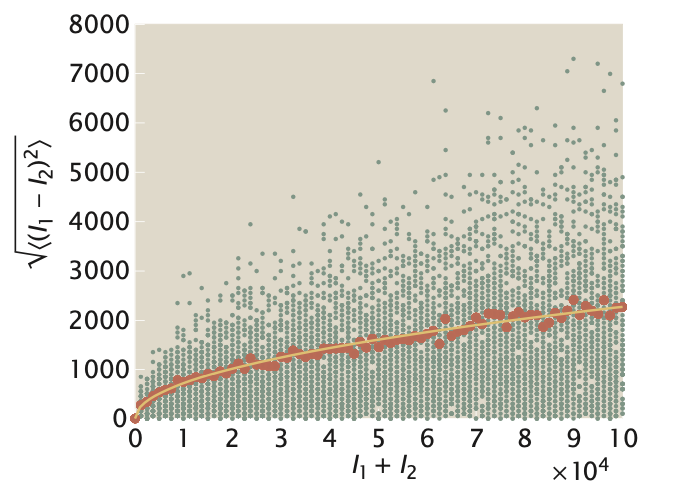
\includegraphics[scale=0.5]{Fig2.11.png}
\end{center}
\caption{Expected simulation results for fluorescence dilution experiment.}
\end{figure}
\part[5] Use a curve fitting function to fit the value of $\alpha$ to the data generated by your simulation to demonstrate that you can recover the value of $\alpha$ you used to generate the data.
\part[5] Now use this function to infer the value of $\alpha$ for the dataset provided with the assignment. Make a plot of data with the fit and showing the obtained value of $\alpha$ and the 95\% confidence interval. 
\end{parts}

\question (20 points)
Analysis of 1D Rate Equations
\begin{parts}
\part[5] Determine the maximum growth rate and the value of $N$ at which maximal growth occurs in the logistic growth equation, $\frac{dN}{dt} = rN\left( 1- N/K\right)$.

\part[10] Consider the following differential equation for expression of a gene X under positive autoregulation:
$$\frac{dX}{dt} = \beta \frac{X^n}{K^n + X^n}  - \alpha X.$$ 
Taking $\alpha=1$, $\beta=10$, $K=5$, and $n=6$, make a rate balance plot as shown in class for the logistic growth equation for positive autoregulation. Identify the steady states and indicate their stability.
\part[5] Plot trajectories that start from the points $X=$ 3, 5, 7, and 15 respectively and describe their behavior relative the the fixed points (steady states) of the model.
\part[3] (Bonus) Redo your parts (b) and (c) for $n=1$. How do your results change?
\end{parts}

\question (20 points) Open reading frames in random DNA. 
In this problem, we will compute the probabilities of finding specific DNA sequences in a perfectly random genome, for which we assume that the four different nucleotides appear randomly and with equal probability.
\begin{figure}
\begin{center}
    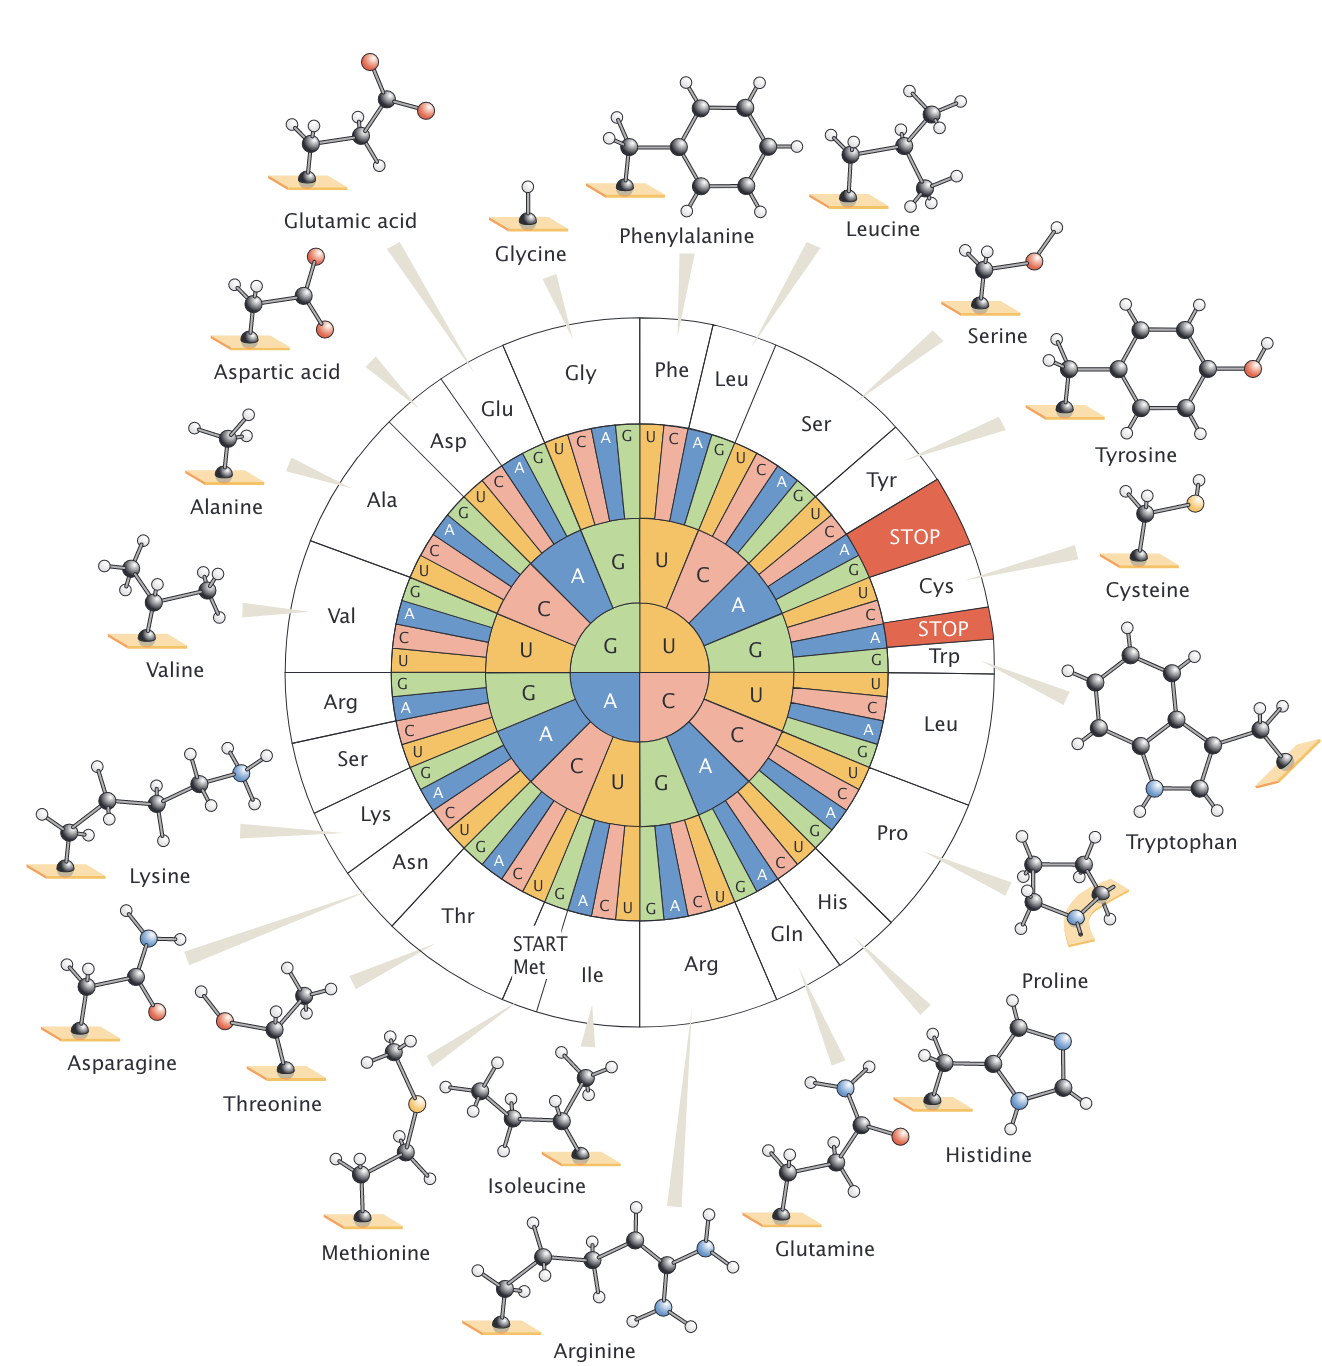
\includegraphics[scale=0.5]{Fig1.4.png}
\end{center}
\caption{The genetic code. \bf{Physical Biology of the Cell, 2nd Ed.}}
\label{fig:genetic code}
\end{figure}
\begin{parts}
\part[5] From the genetic code shown in Fig.~\ref{fig:genetic code}, compute the probability that a randomly chosen sequence of three nucleotides will correspond to a stop codon. Similarly, what is the probability of a randomly chosen sequence corresponding to a start codon? 
\part[5] A reading frame refers to one of three possible ways that a sequence of DNA can be divided into consecutive triplets of nucleotides. An open reading frame (ORF) is a reading frame that contains a start codon and does not contain a stop codon for at least some minimal length of codons. Derive a formula for the probability that a random ORF has a length of $N$ codons (not including the stop codon).
\part[5] Given this probability distribution what is the \emph{average} length of a protein in a random genome?
\part[5] Given that the genome of \emph{E.\ coli} is circular and approximately $5\times 10^6$ bp long, how many ORFs of 30 codons or more to you expect to find? How many ORFs of 300 codons or more do you expect to find? Write a short paragraph speculating about the significance of these results. 
\part[7] (Bonus) Write a simulation code to verify your findings in (d).
\end{parts}



\end{questions}



\end{document}
